\documentclass[landscape,a4paper,10pt]{article}
\usepackage{tikz}
\usepackage{verbatim}
\usepackage[landscape,margin=15mm]{geometry}
\usetikzlibrary{shapes,arrows,fit,calc,positioning}
\begin{document}
File created by KisTA library

Author: F.Herrera

Institution: KTH (2012-2014, Jul), Univ. of Cantabria (from 2014, Sept.)

Rights reserved by the authors in the terms defined by the KisTA license.

KisTA library compilation date: Jul  6 2016 at 13:52:50.

Tracing Options used:
Style=Clustered, Compact; Baselines sep.=1; Max. t span=3; Scale:=0.750000; Landscape; Show sched. activity.
\\
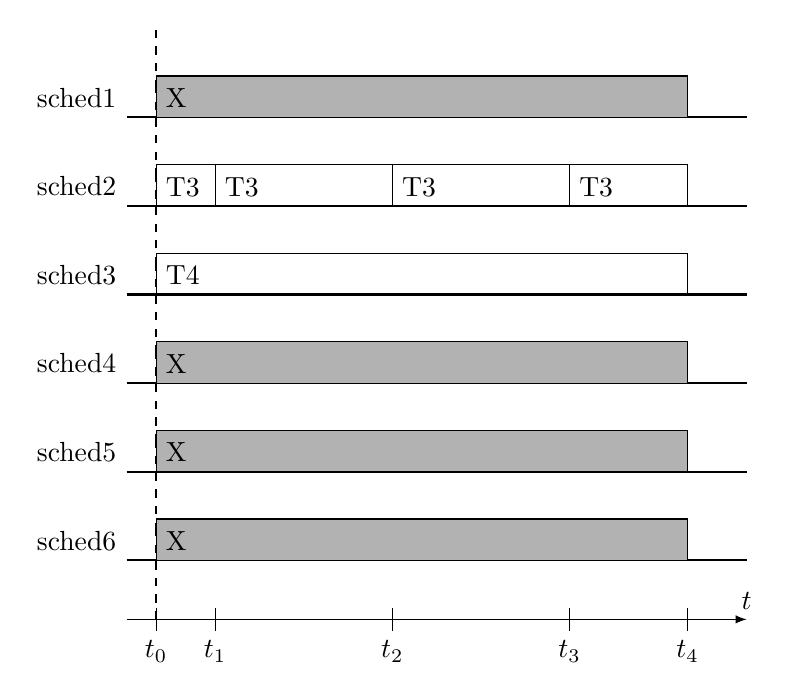
\begin{tikzpicture}[scale=0.750000]
% Draw time axis
% --------------
\draw [-latex](-0.5,0) coordinate(LEFTX)-- (0,0) coordinate (ORIG) -- (10,0) coordinate(RIGHTX) node[above]{$t$};

% Draw time axis divisions
% ------------------------
\draw[] (0,0.2) -- (0,-0.2)  node[below]{$t_{0}$};
\draw[] (1,0.2) -- (1,-0.2)  node[below]{$t_{1}$};
\draw[] (4,0.2) -- (4,-0.2)  node[below]{$t_{2}$};
\draw[] (7,0.2) -- (7,-0.2)  node[below]{$t_{3}$};
\draw[] (9,0.2) -- (9,-0.2)  node[below]{$t_{4}$};

% Draw y axis
% --------------
\draw [dashed,thick]  (ORIG) -- (0,1)coordinate(sched6e0)  -- ++(0,0.5) coordinate(CLUSTER_0_YTOP);

\draw [dashed,thick]  (CLUSTER_0_YTOP) -- ++(0,1) coordinate(sched5e0)  -- ++(0,0.5) coordinate(CLUSTER_1_YTOP);

\draw [dashed,thick]  (CLUSTER_1_YTOP) -- ++(0,1) coordinate(sched4e0)  -- ++(0,0.5) coordinate(CLUSTER_2_YTOP);

\draw [dashed,thick]  (CLUSTER_2_YTOP) -- ++(0,1) coordinate(sched3e0)  -- ++(0,0.5) coordinate(CLUSTER_3_YTOP);

\draw [dashed,thick]  (CLUSTER_3_YTOP) -- ++(0,1) coordinate(sched2e0)  -- ++(0,0.5) coordinate(CLUSTER_4_YTOP);

\draw [dashed,thick]  (CLUSTER_4_YTOP) -- ++(0,1) coordinate(sched1e0)  -- ++(0,0.5) coordinate(CLUSTER_5_YTOP);

\draw [dashed,thick] (CLUSTER_5_YTOP) -- ++(0,1) coordinate(YTOP);

% Draw baselines
% --------------
\draw [thick] (LEFTX|-sched6e0) node[above left]{sched6} -- (sched6e0-|RIGHTX);

\draw [thick] (LEFTX|-sched5e0) node[above left]{sched5} -- (sched5e0-|RIGHTX);

\draw [thick] (LEFTX|-sched4e0) node[above left]{sched4} -- (sched4e0-|RIGHTX);

\draw [thick] (LEFTX|-sched3e0) node[above left]{sched3} -- (sched3e0-|RIGHTX);

\draw [thick] (LEFTX|-sched2e0) node[above left]{sched2} -- (sched2e0-|RIGHTX);

\draw [thick] (LEFTX|-sched1e0) node[above left]{sched1} -- (sched1e0-|RIGHTX);

% Set event coordinates   
% ------------------------
\path (sched6e0) ++ (9,0) coordinate(sched6e4);
\path (sched5e0) ++ (9,0) coordinate(sched5e4);
\path (sched4e0) ++ (9,0) coordinate(sched4e4);
\path (sched3e0) ++ (9,0) coordinate(sched3e4);
\path (sched2e0) ++ (1,0) coordinate(sched2e1) ++ (3,0) coordinate(sched2e2) ++ (3,0) coordinate(sched2e3) ++ (2,0) coordinate(sched2e4);
\path (sched1e0) ++ (9,0) coordinate(sched1e4);

% Draw scheduler activity (relying on event coordinates) 
% -------------------------------------------------------
\begin{scope}[shift={(sched6e0)}]
\draw[fill=black!30] (0,0) rectangle (9,0.7);
\draw[] (0,0) node[rectangle, above right] {X};
\end{scope}
\begin{scope}[shift={(sched5e0)}]
\draw[fill=black!30] (0,0) rectangle (9,0.7);
\draw[] (0,0) node[rectangle, above right] {X};
\end{scope}
\begin{scope}[shift={(sched4e0)}]
\draw[fill=black!30] (0,0) rectangle (9,0.7);
\draw[] (0,0) node[rectangle, above right] {X};
\end{scope}
\begin{scope}[shift={(sched3e0)}]
\draw[] (0,0) rectangle (9,0.7);
\draw[] (0,0) node[rectangle, above right] {T4};
\end{scope}
\begin{scope}[shift={(sched2e0)}]
\draw[] (0,0) rectangle (1,0.7);
\draw[] (0,0) node[rectangle, above right] {T3};
\end{scope}
\begin{scope}[shift={(sched2e1)}]
\draw[] (0,0) rectangle (3,0.7);
\draw[] (0,0) node[rectangle, above right] {T3};
\end{scope}
\begin{scope}[shift={(sched2e2)}]
\draw[] (0,0) rectangle (3,0.7);
\draw[] (0,0) node[rectangle, above right] {T3};
\end{scope}
\begin{scope}[shift={(sched2e3)}]
\draw[] (0,0) rectangle (2,0.7);
\draw[] (0,0) node[rectangle, above right] {T3};
\end{scope}
\begin{scope}[shift={(sched1e0)}]
\draw[fill=black!30] (0,0) rectangle (9,0.7);
\draw[] (0,0) node[rectangle, above right] {X};
\end{scope}
\end{tikzpicture}

% Show Automatic Task Alias names 
% --------------------------------
\textbf{Task alias list (alias=task name):}\\
T6=T7 , 
T5=T6 , 
T4=T5 , 
T7=T8 , 
T3=T4 , 
T1=T2 , 
T2=T3 , 
T0=T1\\

% Show Time stamp values
% ---------------------
\textbf{Time Stamp values:}\\
$t_{0} = 9 ms; t_{1} = 9006860 ns; t_{2} = 9694560 ns; t_{3} = 10382260 ns; t_{4} = 10758059674 ps;  \\
$

% Show Time span values
% ---------------------
\textbf{Time Span values:}\\
$t_{1} - t_{0} = 6860 ns; t_{2} - t_{1} = 687700 ns; t_{3} - t_{2} = 687700 ns; t_{4} - t_{3} = 375799674 ps;  \\
$

\end{document}

